
            \documentclass[8pt]{beamer} 
            \usetheme{CambridgeUS} 
            \usepackage{textpos} 
            \usepackage[latin1]{inputenc} 
            \usepackage{amsmath} 
            \usepackage{mathtools} 
            \usepackage{color} 
            \usepackage{mathabx} 
            \usepackage{graphicx} 
            \usepackage{tikz} 
            \usepackage{esvect} 
            \usetikzlibrary{arrows,shapes} 
            \usecolortheme{beaver} 
            \usepackage{graphicx} 
            \usepackage{changepage} 
            \setbeamertemplate{navigation symbols}{} 
            \setbeamertemplate{navigation symbols}{} 
        
        \title{GEANT4 Simulation Report}
        \author{Riccardo Nicolaidis \footnote{riccardo.nicolaidis@unitn.it}}
        \date{\today}
        
        \begin{document}
        
        \begin{frame}
            \titlepage
        \end{frame}
        
        \begin{frame}
            \frametitle{Montecarlo quantities for electrons}
        
        \begin{figure}[h]
            \centering
            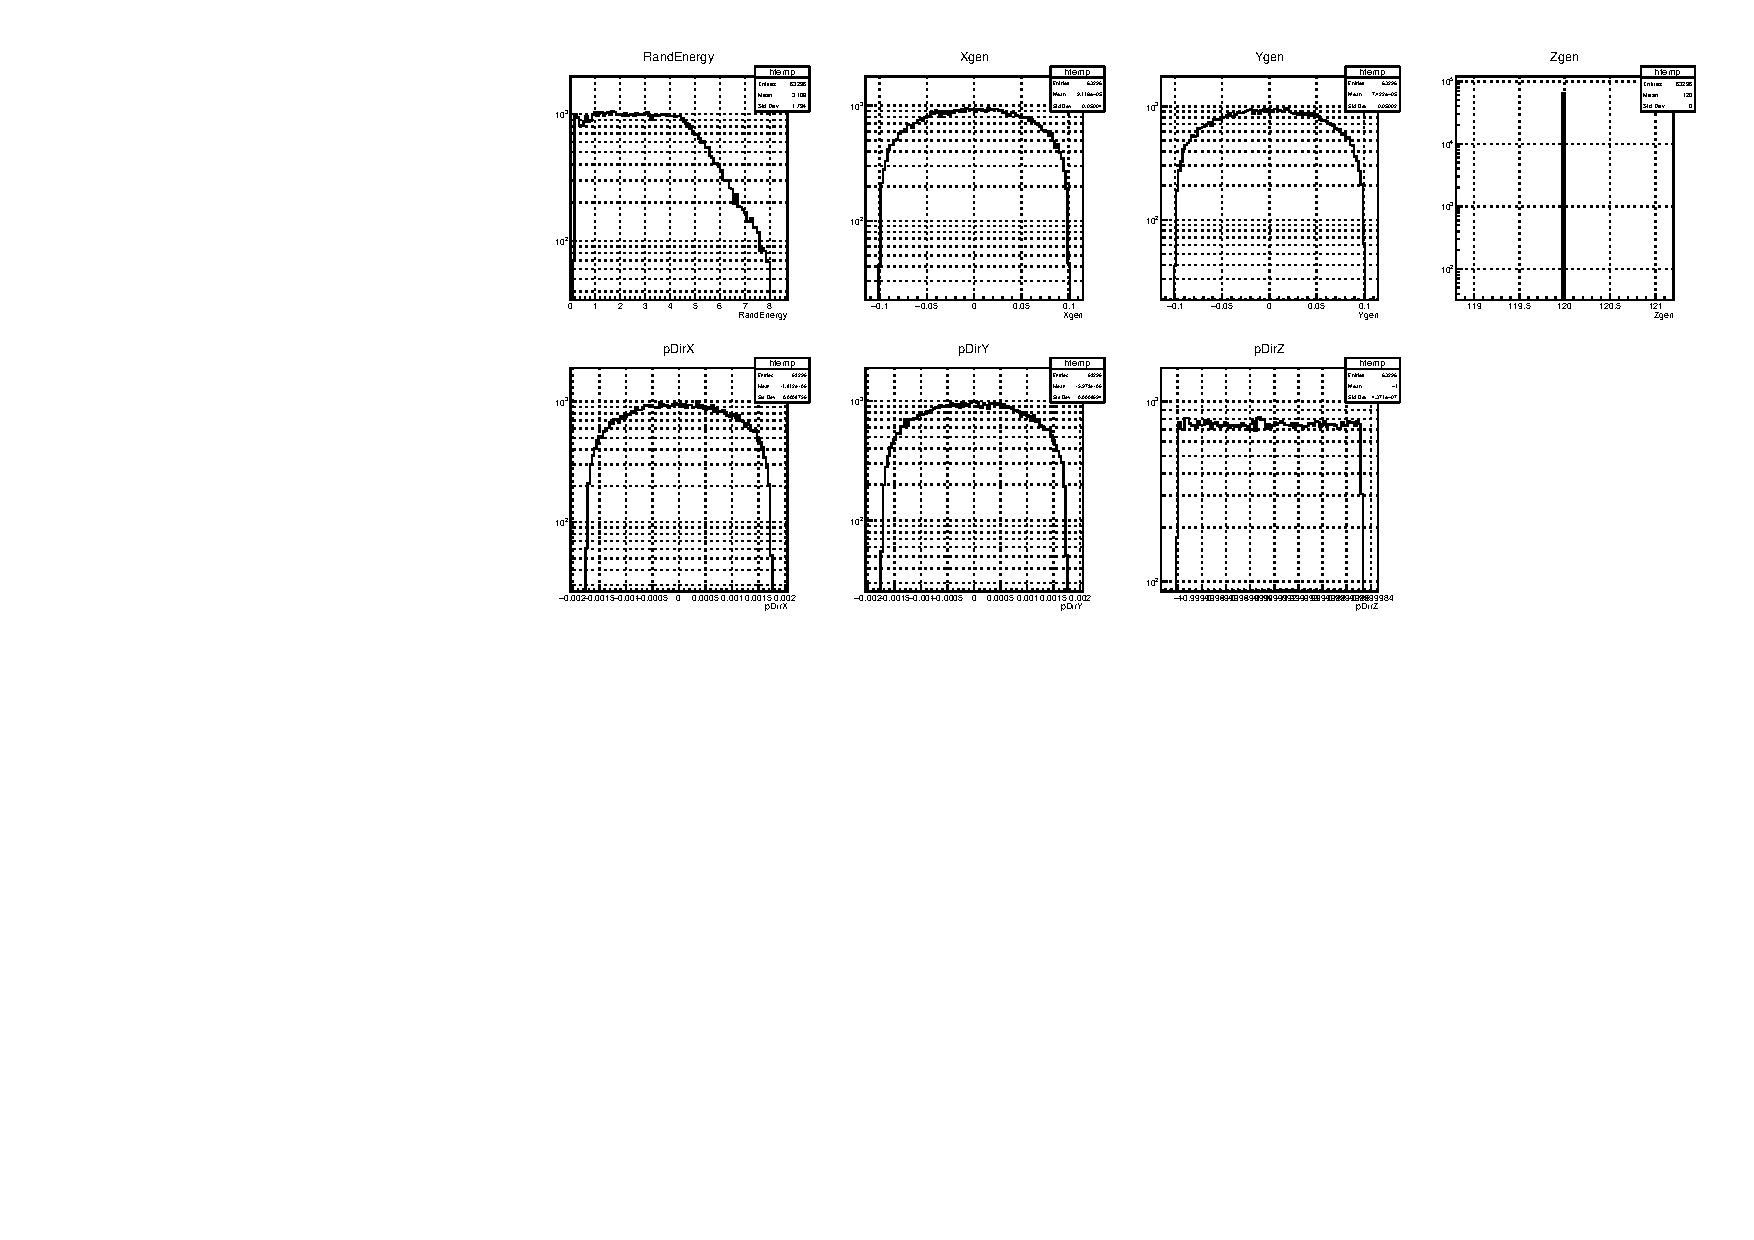
\includegraphics[width=0.8\textwidth]{/home/riccardo/Documenti/GeantProjects/LEM_GDML_upgrade/Output_Geant4Simulation_20230615_Old/Analysis_output/GDML_file_0/Montecarlo_e-_t0.pdf}
            \caption{MC quantities}
        \end{figure}
        
        \end{frame}
        
        \begin{frame}
            \frametitle{Energies distribution for electrons}
        
        \begin{figure}[h]
            \centering
            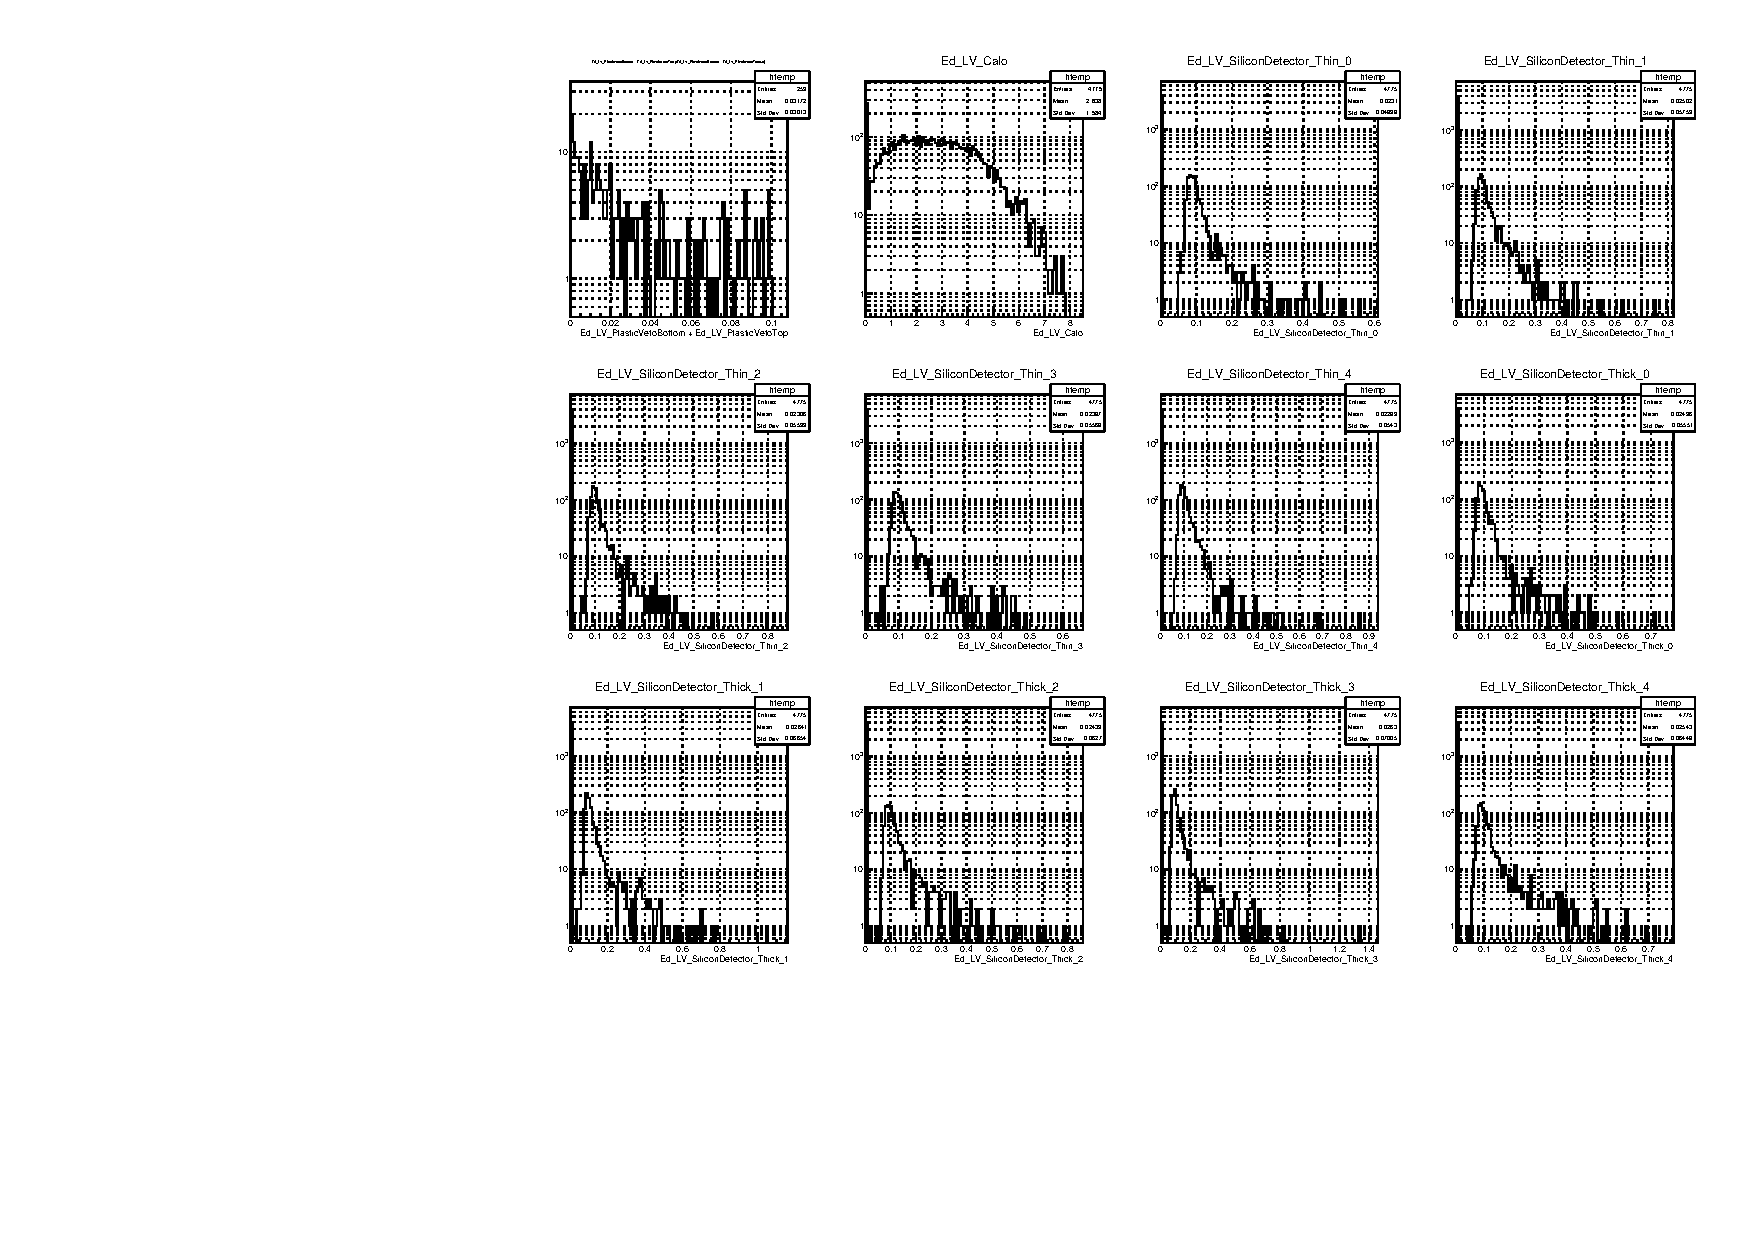
\includegraphics[width=0.8\textwidth]{/home/riccardo/Documenti/GeantProjects/LEM_GDML_upgrade/Output_Geant4Simulation_20230615_Old/Analysis_output/GDML_file_0/Energies_e-_t0.pdf}
            \caption{Detected energies}
        \end{figure}
        
        \end{frame}
        
        \begin{frame}
            \frametitle{Angles distribution accepted for electrons}
        
        \begin{figure}[h]
            \centering
            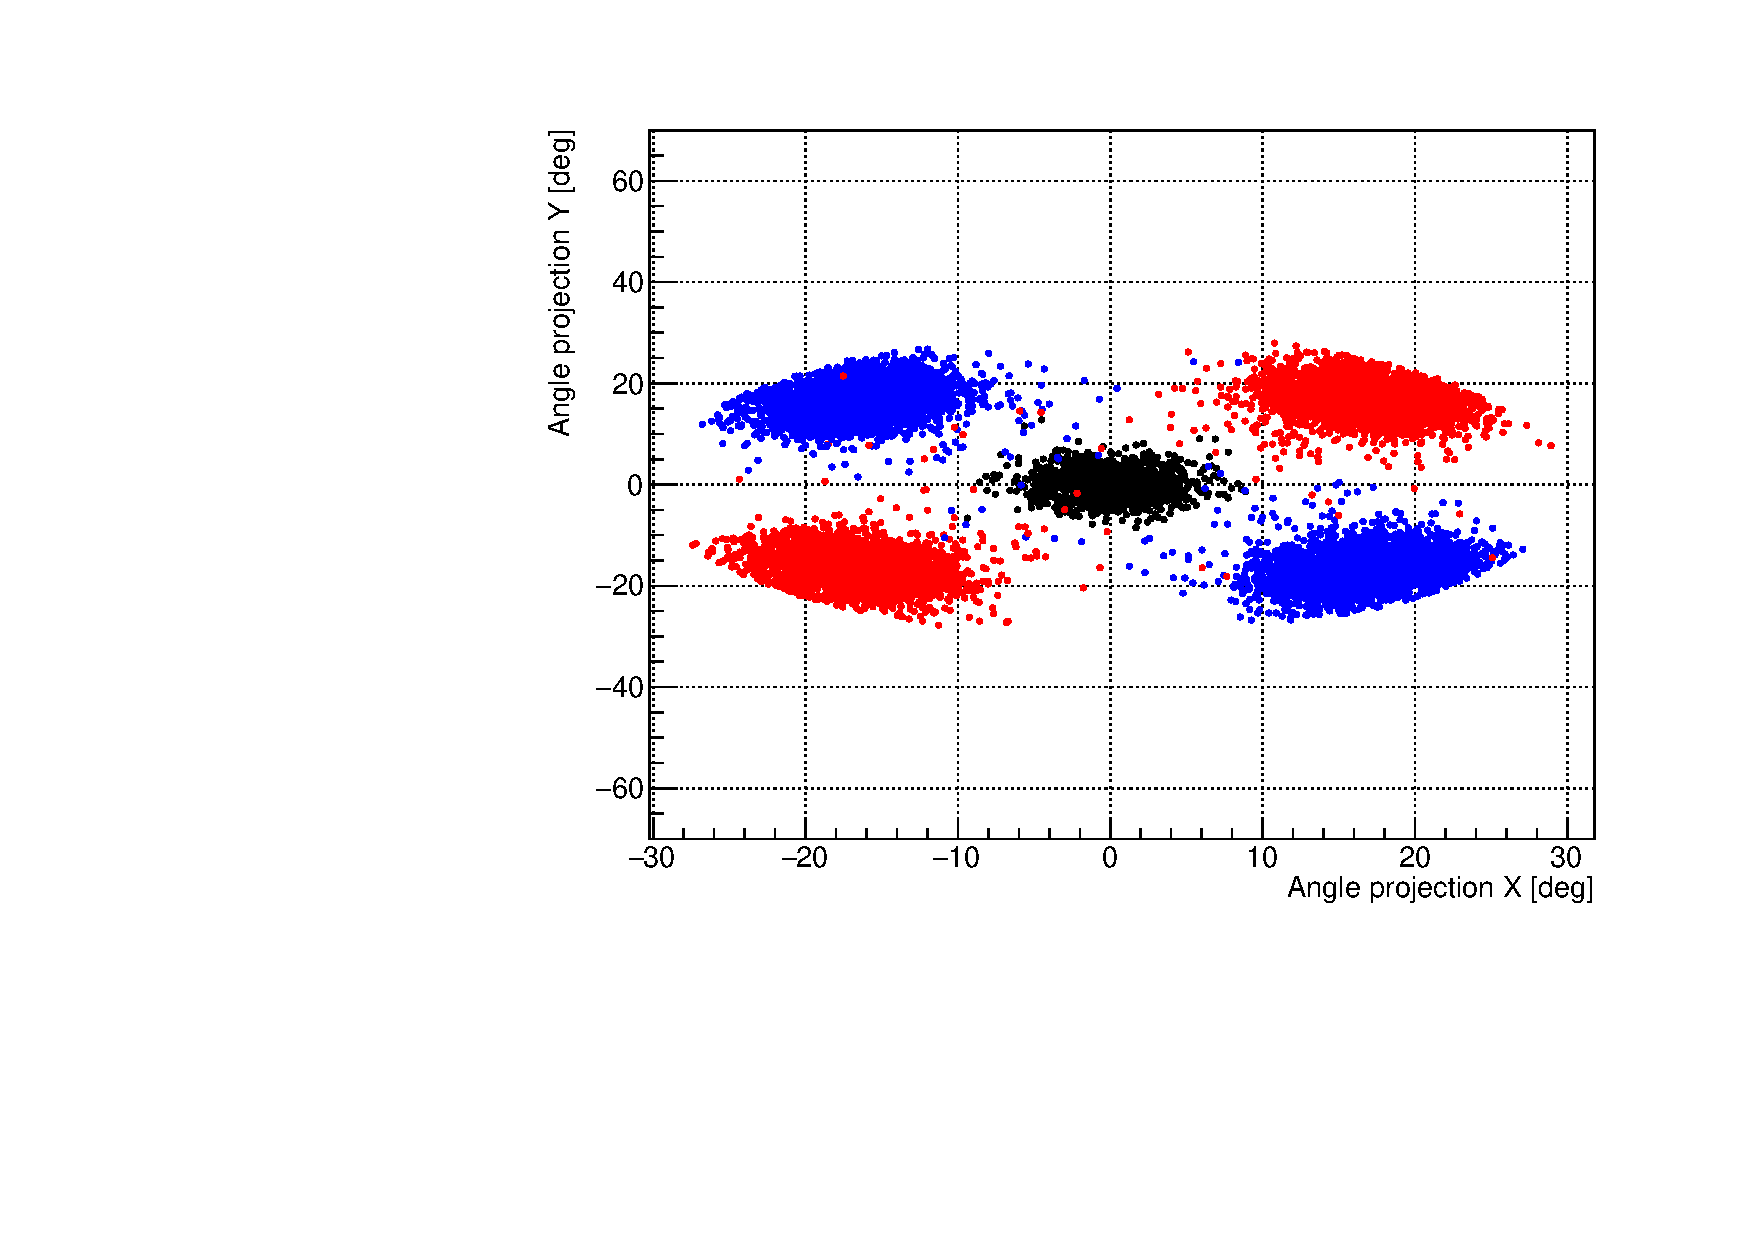
\includegraphics[width=0.8\textwidth]{/home/riccardo/Documenti/GeantProjects/LEM_GDML_upgrade/Output_Geant4Simulation_20230615_Old/Analysis_output/GDML_file_0/Angles_e-_t0.pdf}
            \caption{Angles distribution}
        \end{figure}
        
        \end{frame}
        
        \begin{frame}
            \frametitle{Geometric factors for electrons}
        
        \begin{figure}[h]
            \centering
            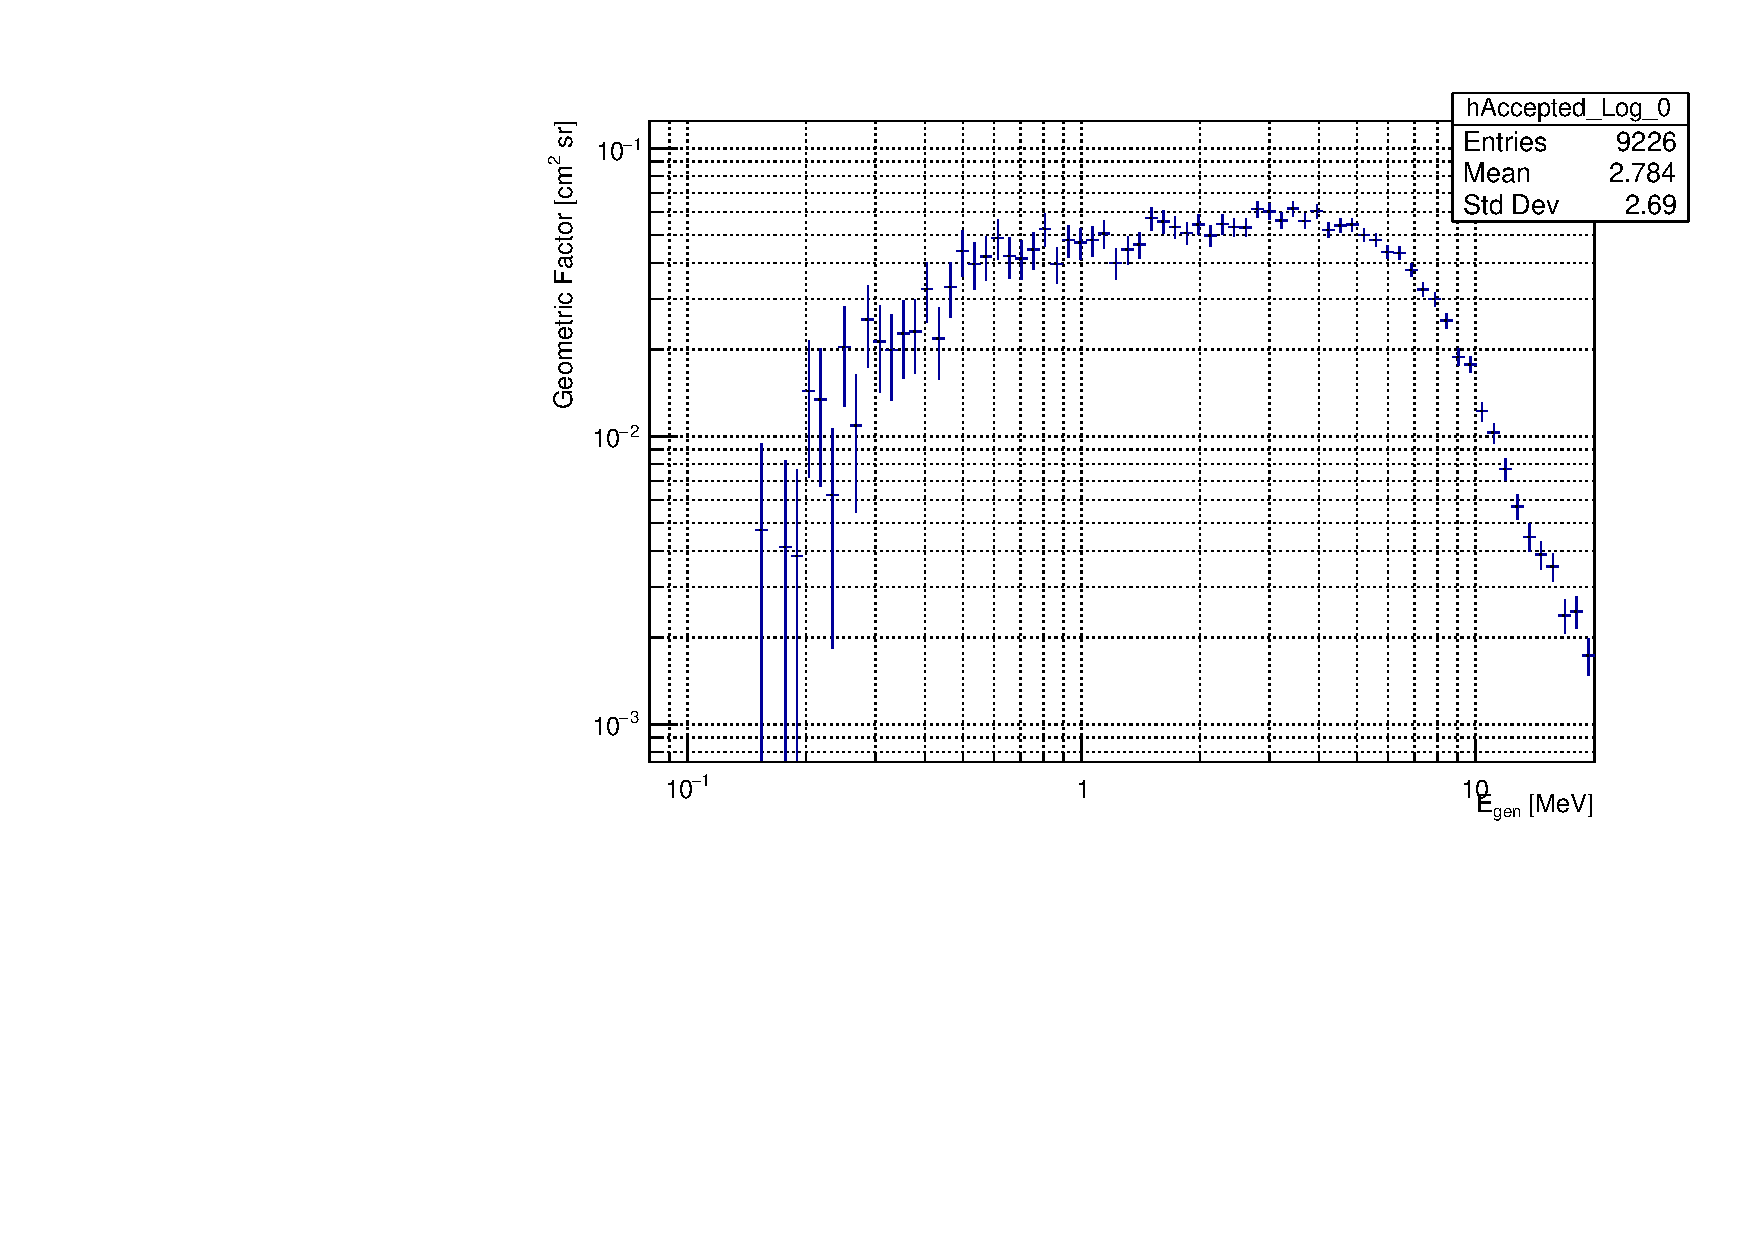
\includegraphics[width=0.8\textwidth]{/home/riccardo/Documenti/GeantProjects/LEM_GDML_upgrade/Output_Geant4Simulation_20230615_Old/Analysis_output/GDML_file_0/Acceptances_e-_t0_alias.pdf}
            \caption{Geometric factors}
        \end{figure}
        
        \end{frame}
        
        \begin{frame}
            \frametitle{Geometric factors for electrons}
        
        \begin{figure}[h]
            \centering
            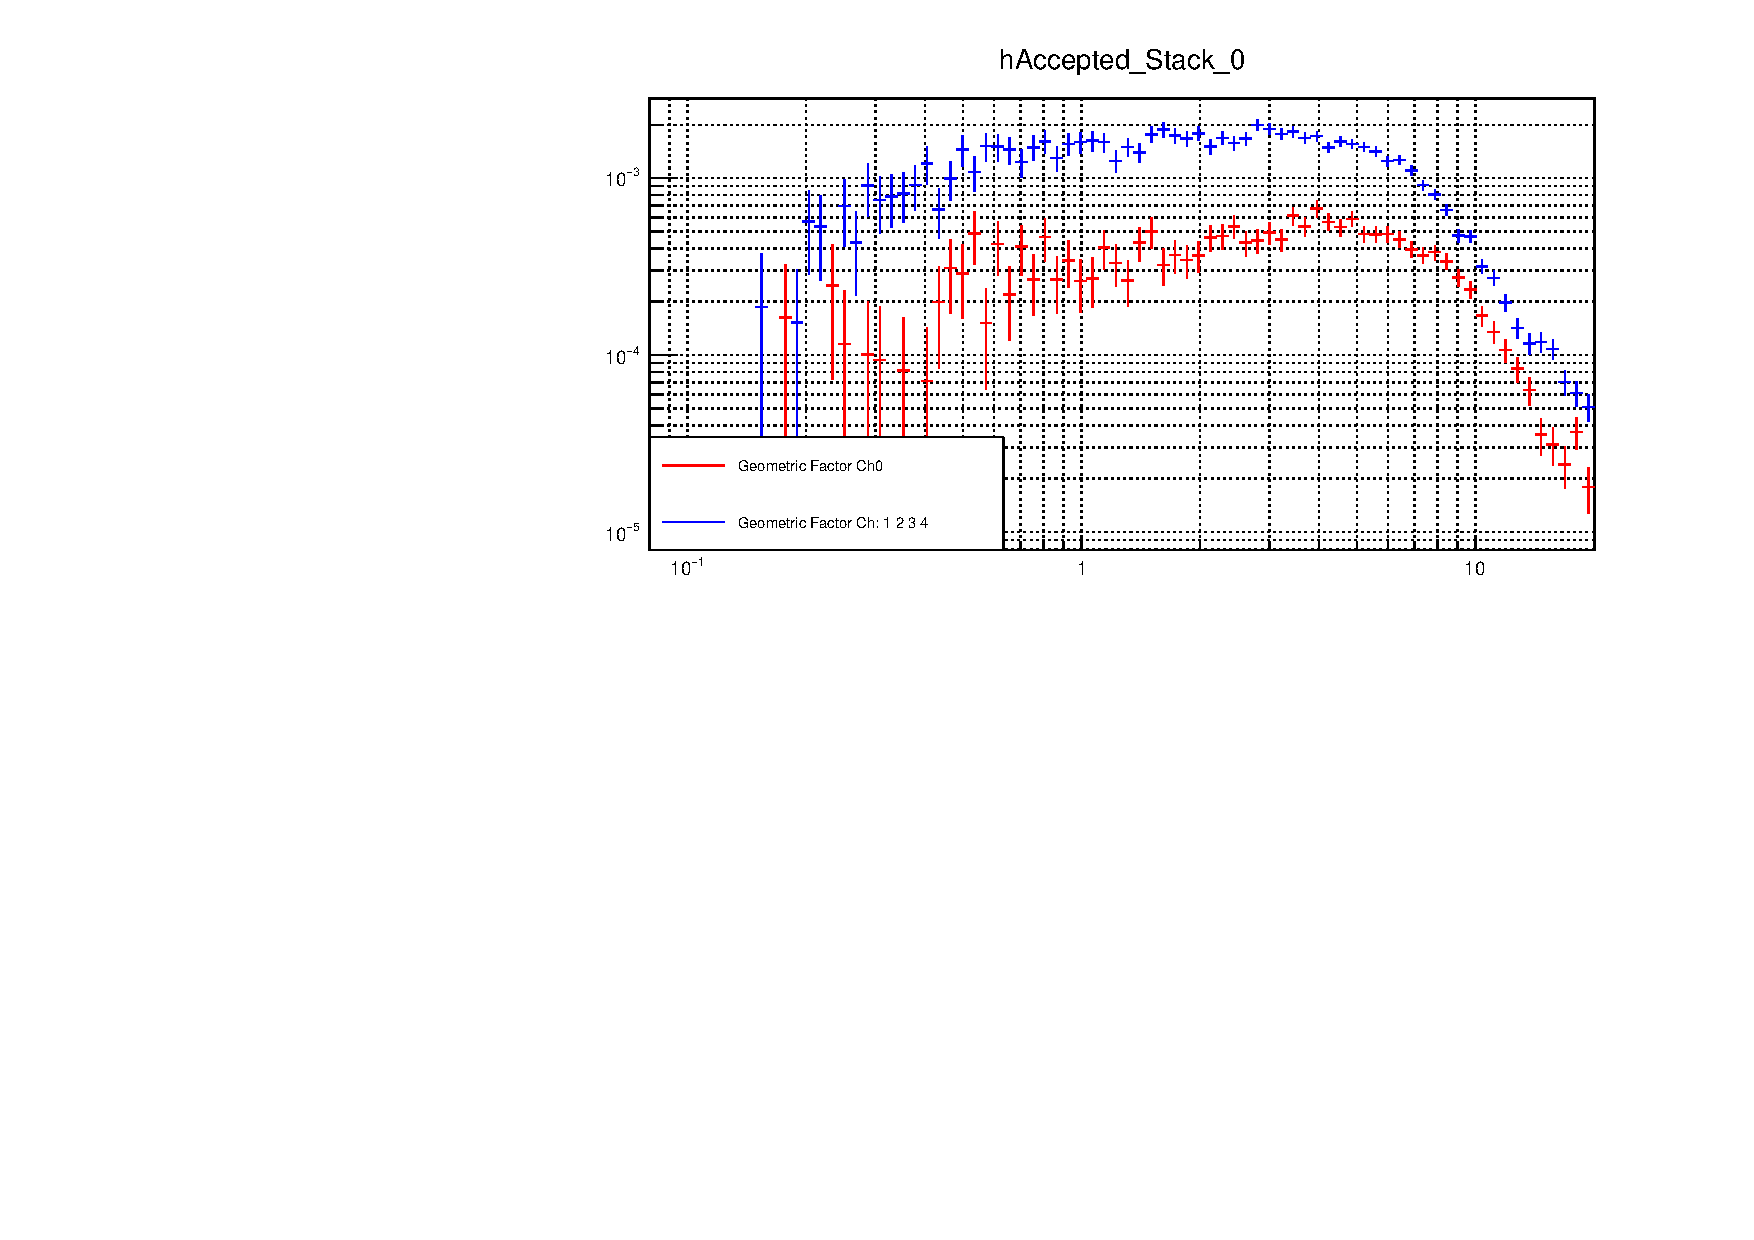
\includegraphics[width=0.8\textwidth]{/home/riccardo/Documenti/GeantProjects/LEM_GDML_upgrade/Output_Geant4Simulation_20230615_Old/Analysis_output/GDML_file_0/ChannelGeomFactor_e-_t0_alias.pdf}
            \caption{Geometric factors}
        \end{figure}
        
        \end{frame}
        
        \begin{frame}
            \frametitle{Montecarlo quantities for protons}
        
        \begin{figure}[h]
            \centering
            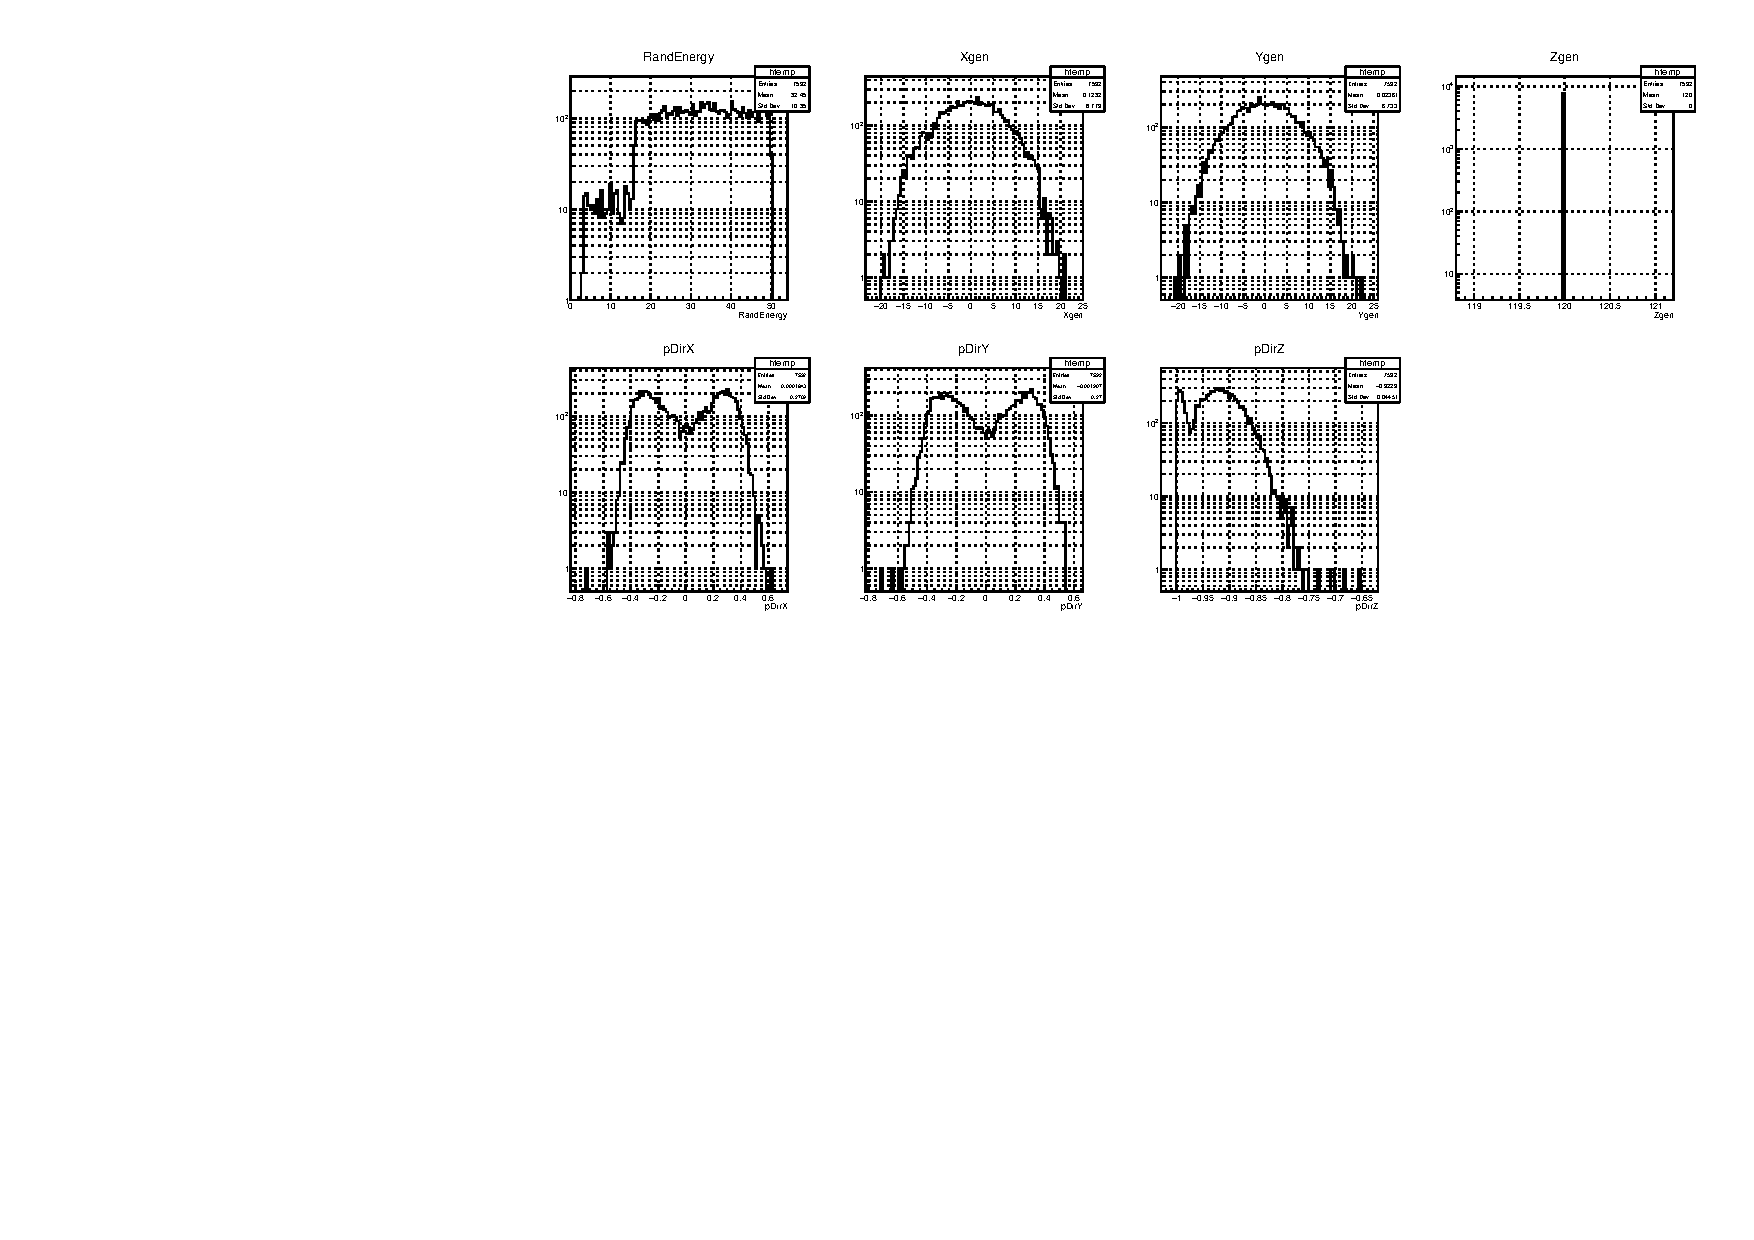
\includegraphics[width=0.8\textwidth]{/home/riccardo/Documenti/GeantProjects/LEM_GDML_upgrade/Output_Geant4Simulation_20230615_Old/Analysis_output/GDML_file_0/Montecarlo_proton_t0.pdf}
            \caption{MC quantities}
        \end{figure}
        
        \end{frame}
        
        \begin{frame}
            \frametitle{Energies distribution for protons}
        
        \begin{figure}[h]
            \centering
            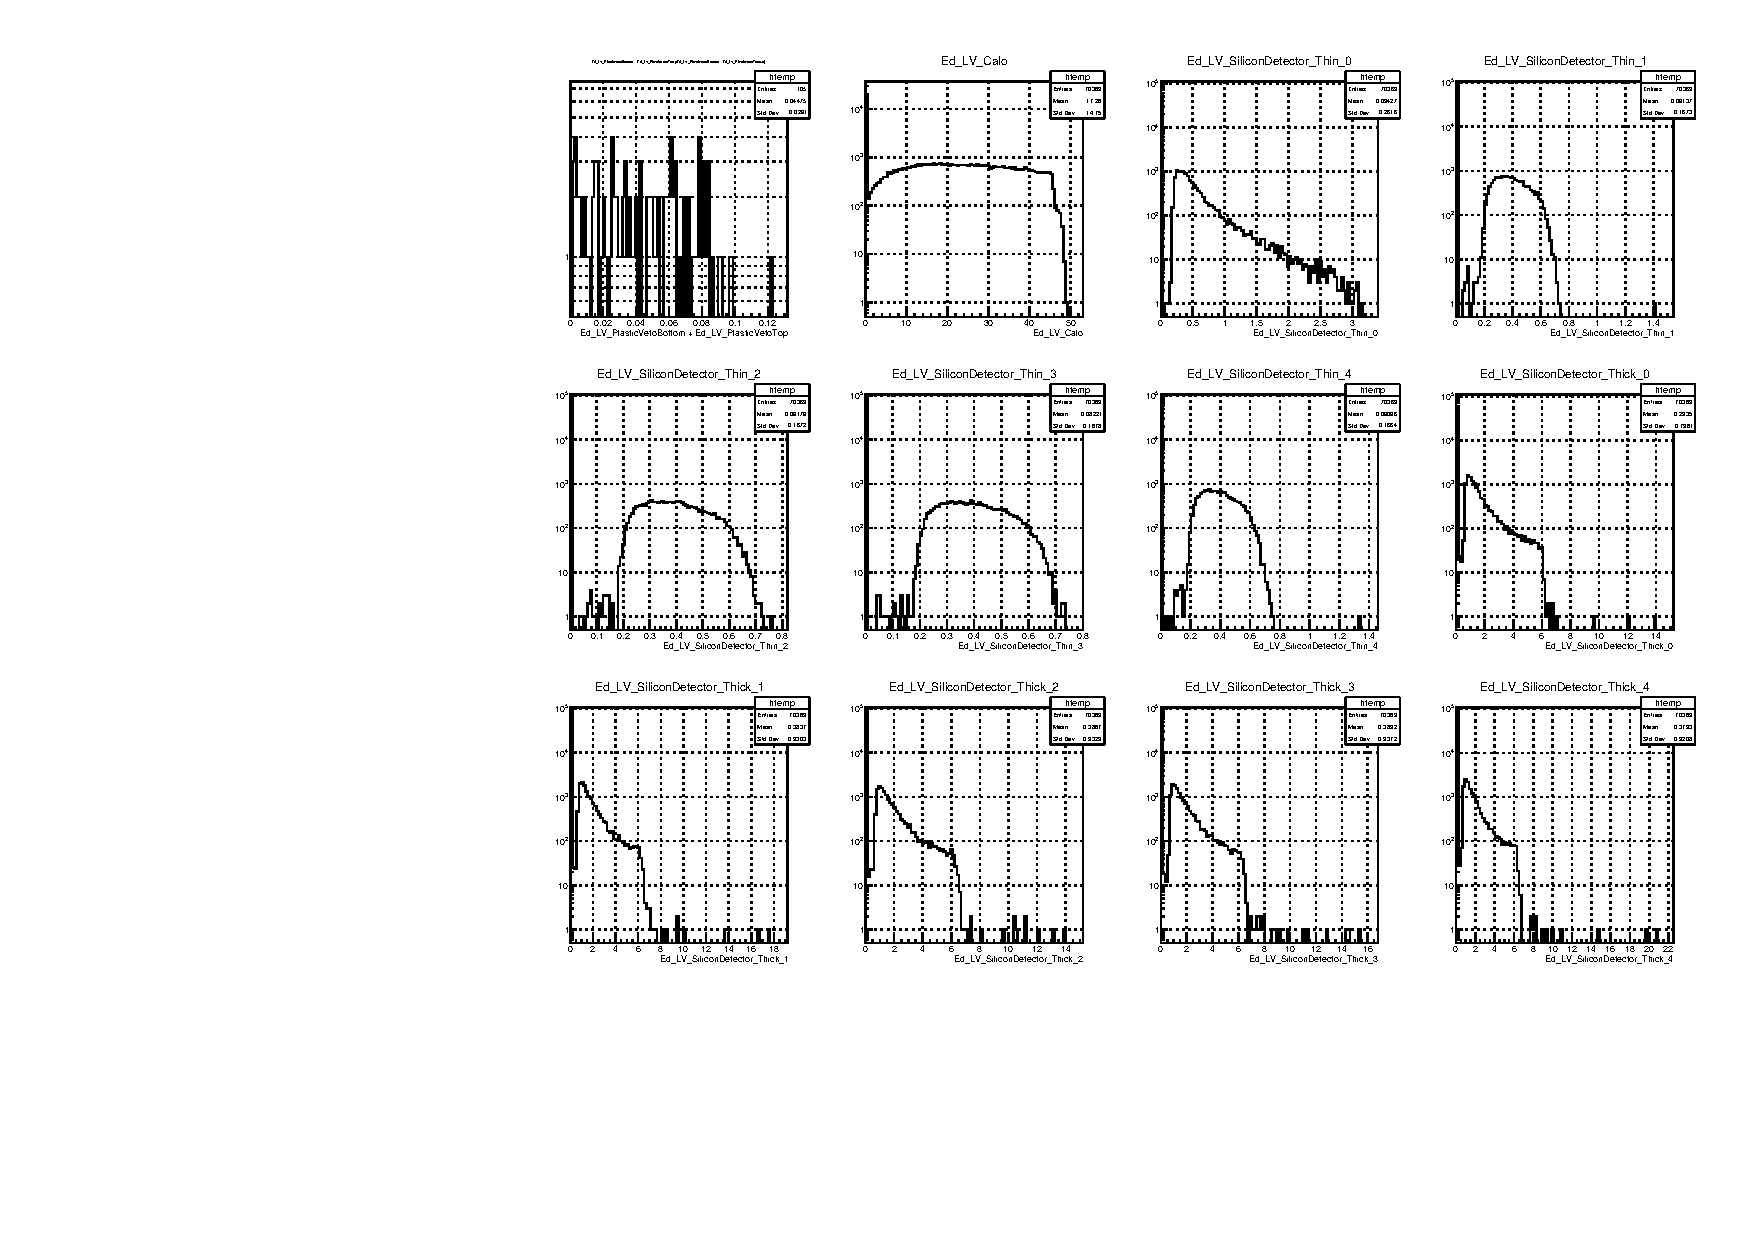
\includegraphics[width=0.8\textwidth]{/home/riccardo/Documenti/GeantProjects/LEM_GDML_upgrade/Output_Geant4Simulation_20230615_Old/Analysis_output/GDML_file_0/Energies_proton_t0.pdf}
            \caption{Detected energies}
        \end{figure}
        
        \end{frame}
        
        \begin{frame}
            \frametitle{Angles distribution accepted for protons}
        
        \begin{figure}[h]
            \centering
            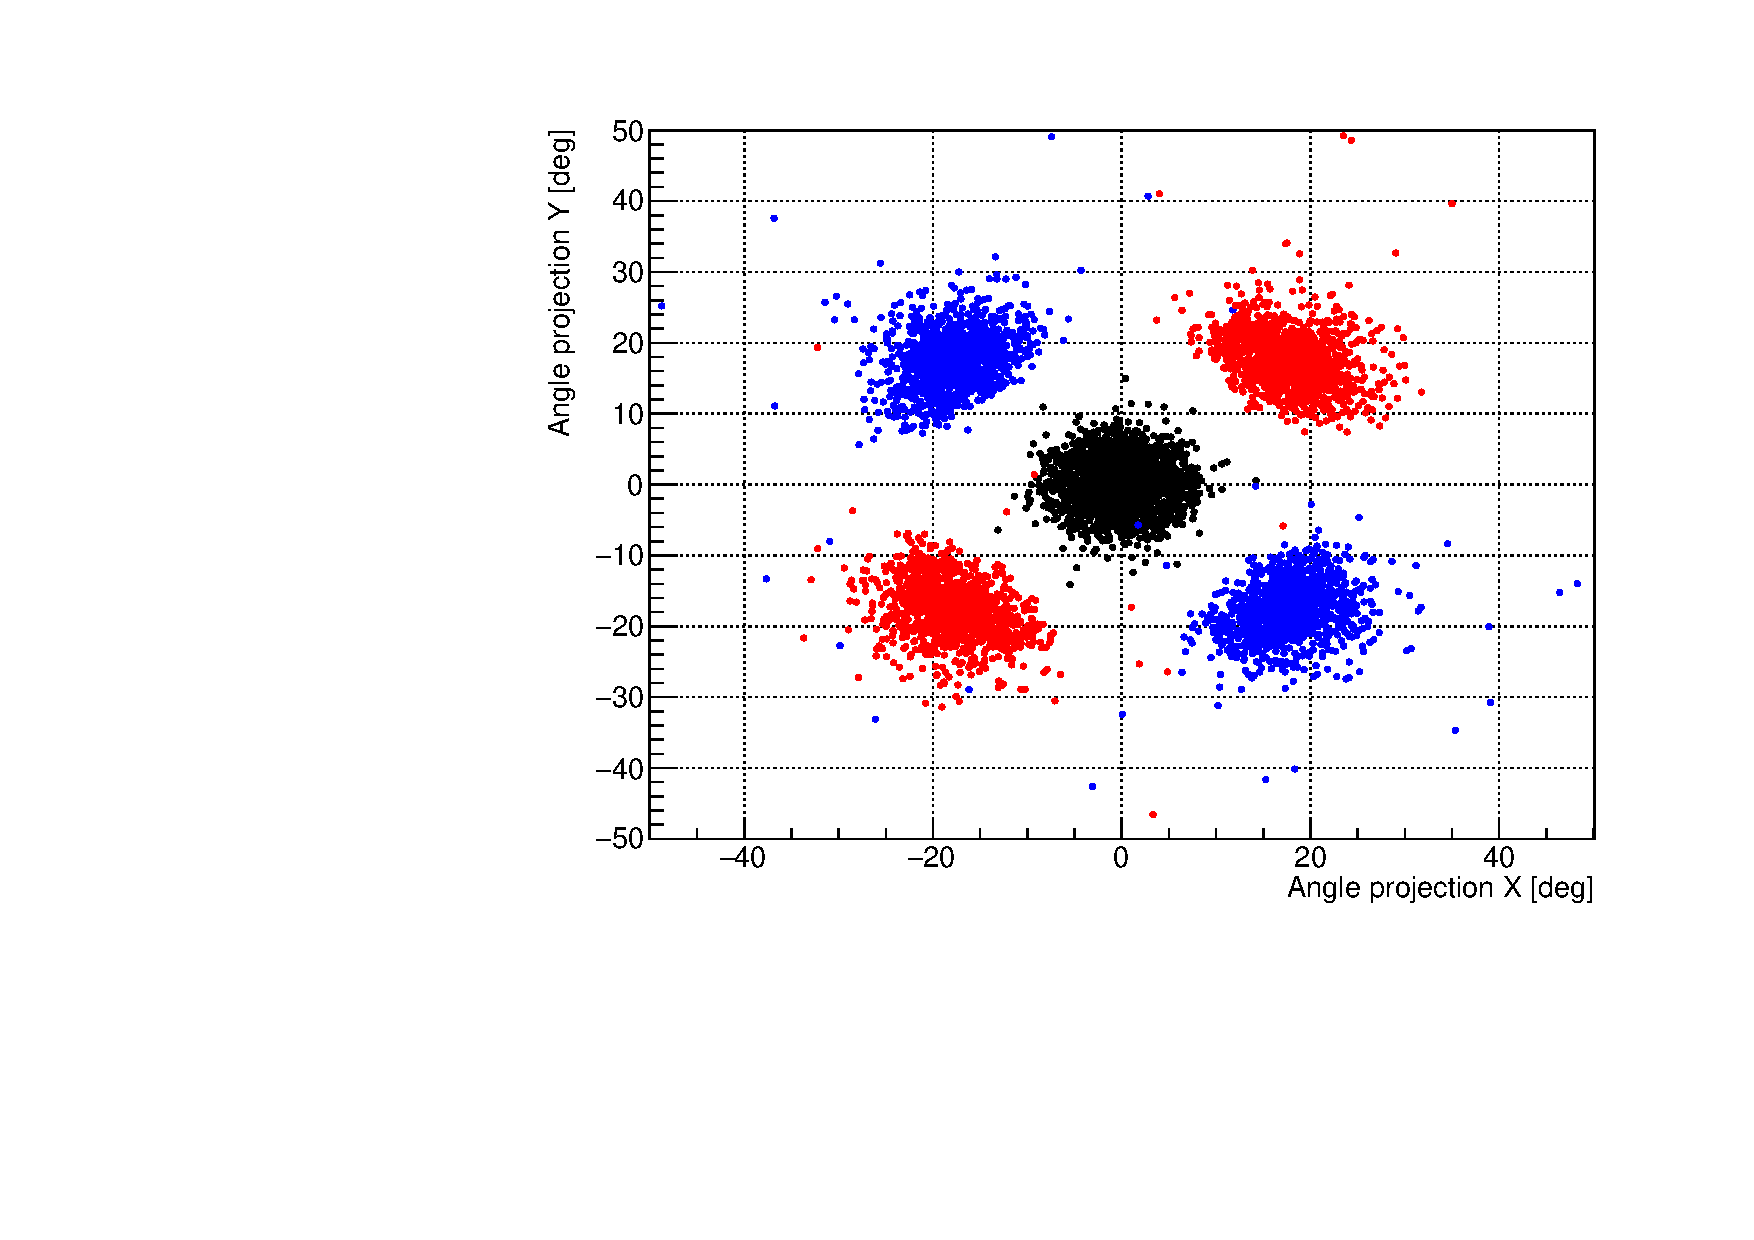
\includegraphics[width=0.8\textwidth]{/home/riccardo/Documenti/GeantProjects/LEM_GDML_upgrade/Output_Geant4Simulation_20230615_Old/Analysis_output/GDML_file_0/Angles_proton_t0.pdf}
            \caption{Angles distribution}
        \end{figure}
        
        \end{frame}
        
        \begin{frame}
            \frametitle{Geometric factors for protons}
        
        \begin{figure}[h]
            \centering
            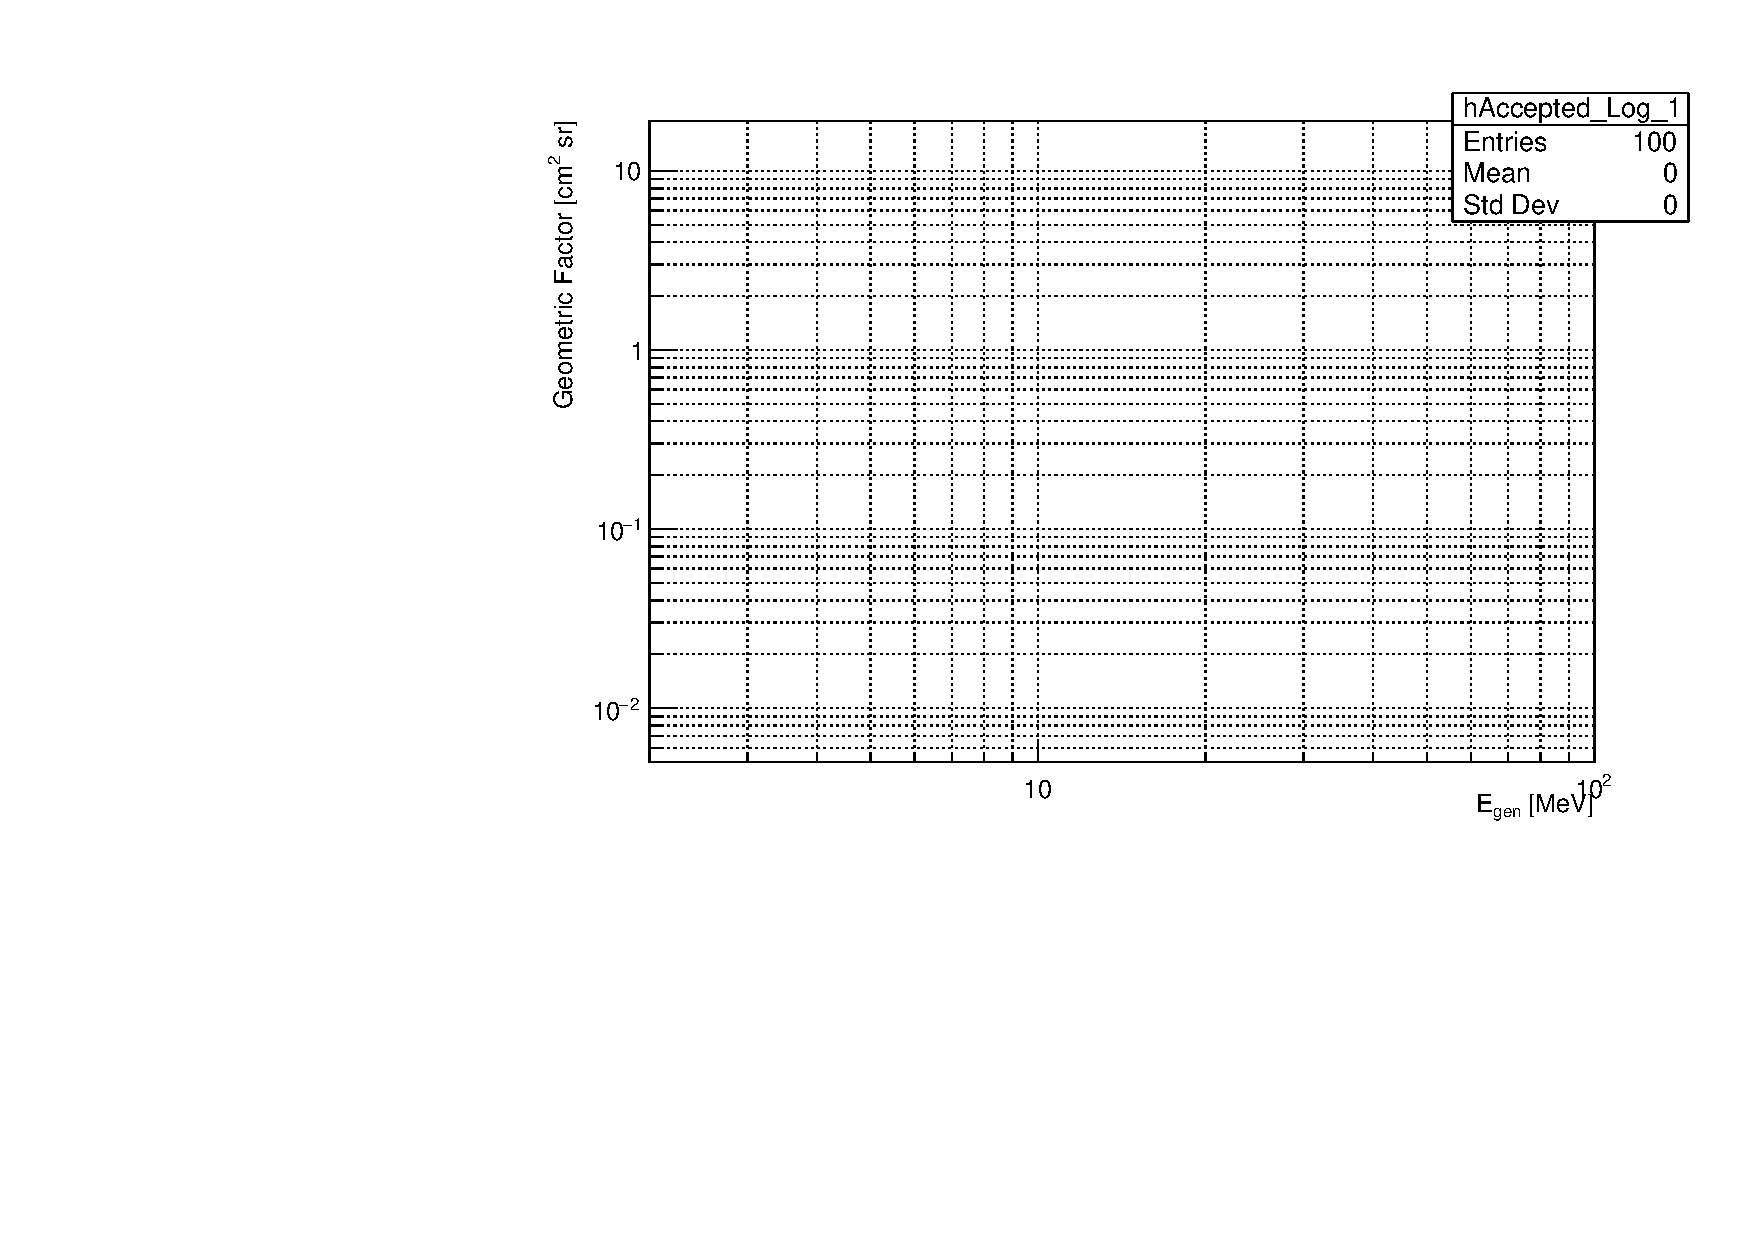
\includegraphics[width=0.8\textwidth]{/home/riccardo/Documenti/GeantProjects/LEM_GDML_upgrade/Output_Geant4Simulation_20230615_Old/Analysis_output/GDML_file_0/Acceptances_proton_t0_alias.pdf}
            \caption{Geometric factors}
        \end{figure}
        
        \end{frame}
        
        \begin{frame}
            \frametitle{Geometric factors for protons}
        
        \begin{figure}[h]
            \centering
            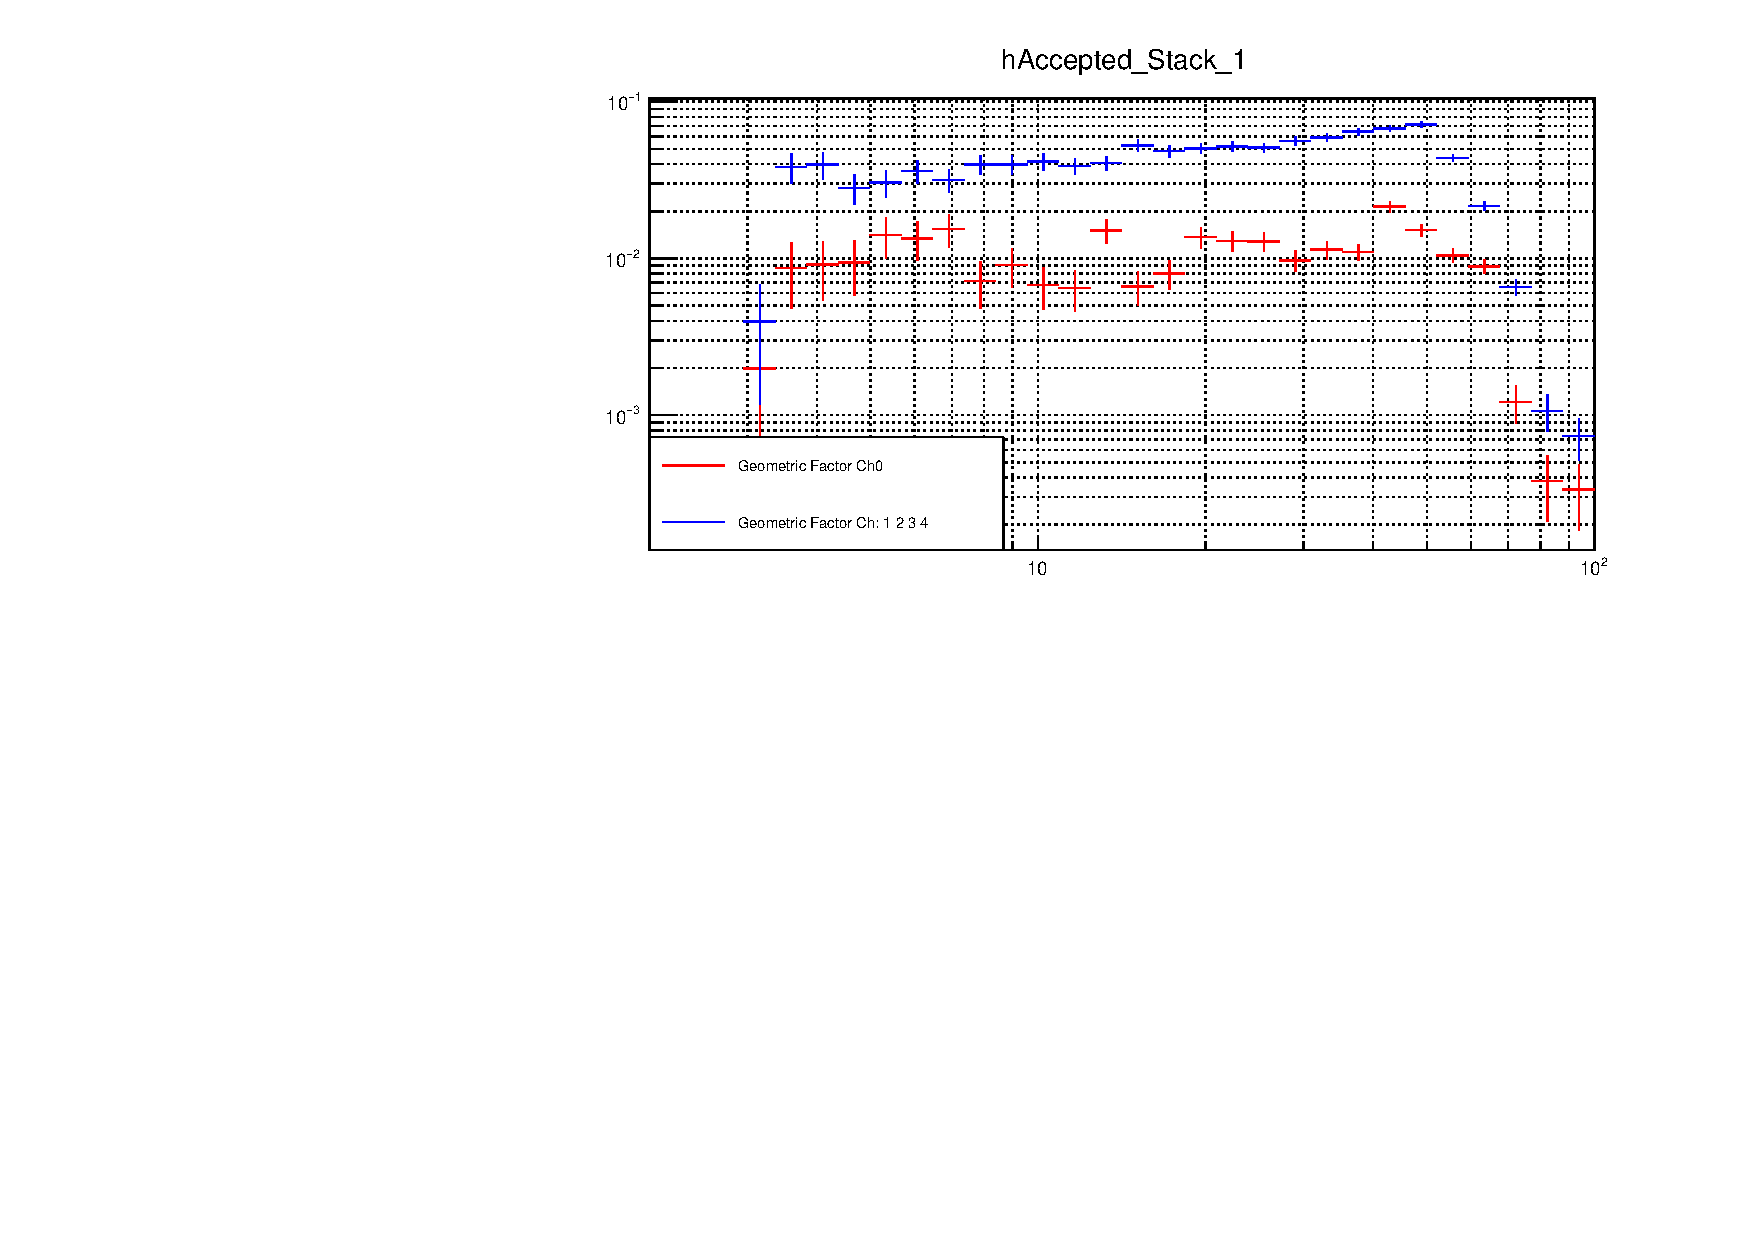
\includegraphics[width=0.8\textwidth]{/home/riccardo/Documenti/GeantProjects/LEM_GDML_upgrade/Output_Geant4Simulation_20230615_Old/Analysis_output/GDML_file_0/ChannelGeomFactor_proton_t0_alias.pdf}
            \caption{Geometric factors}
        \end{figure}
        
        \end{frame}
        
        \begin{frame}
            \frametitle{Montecarlo quantities for alphas}
        
        \begin{figure}[h]
            \centering
            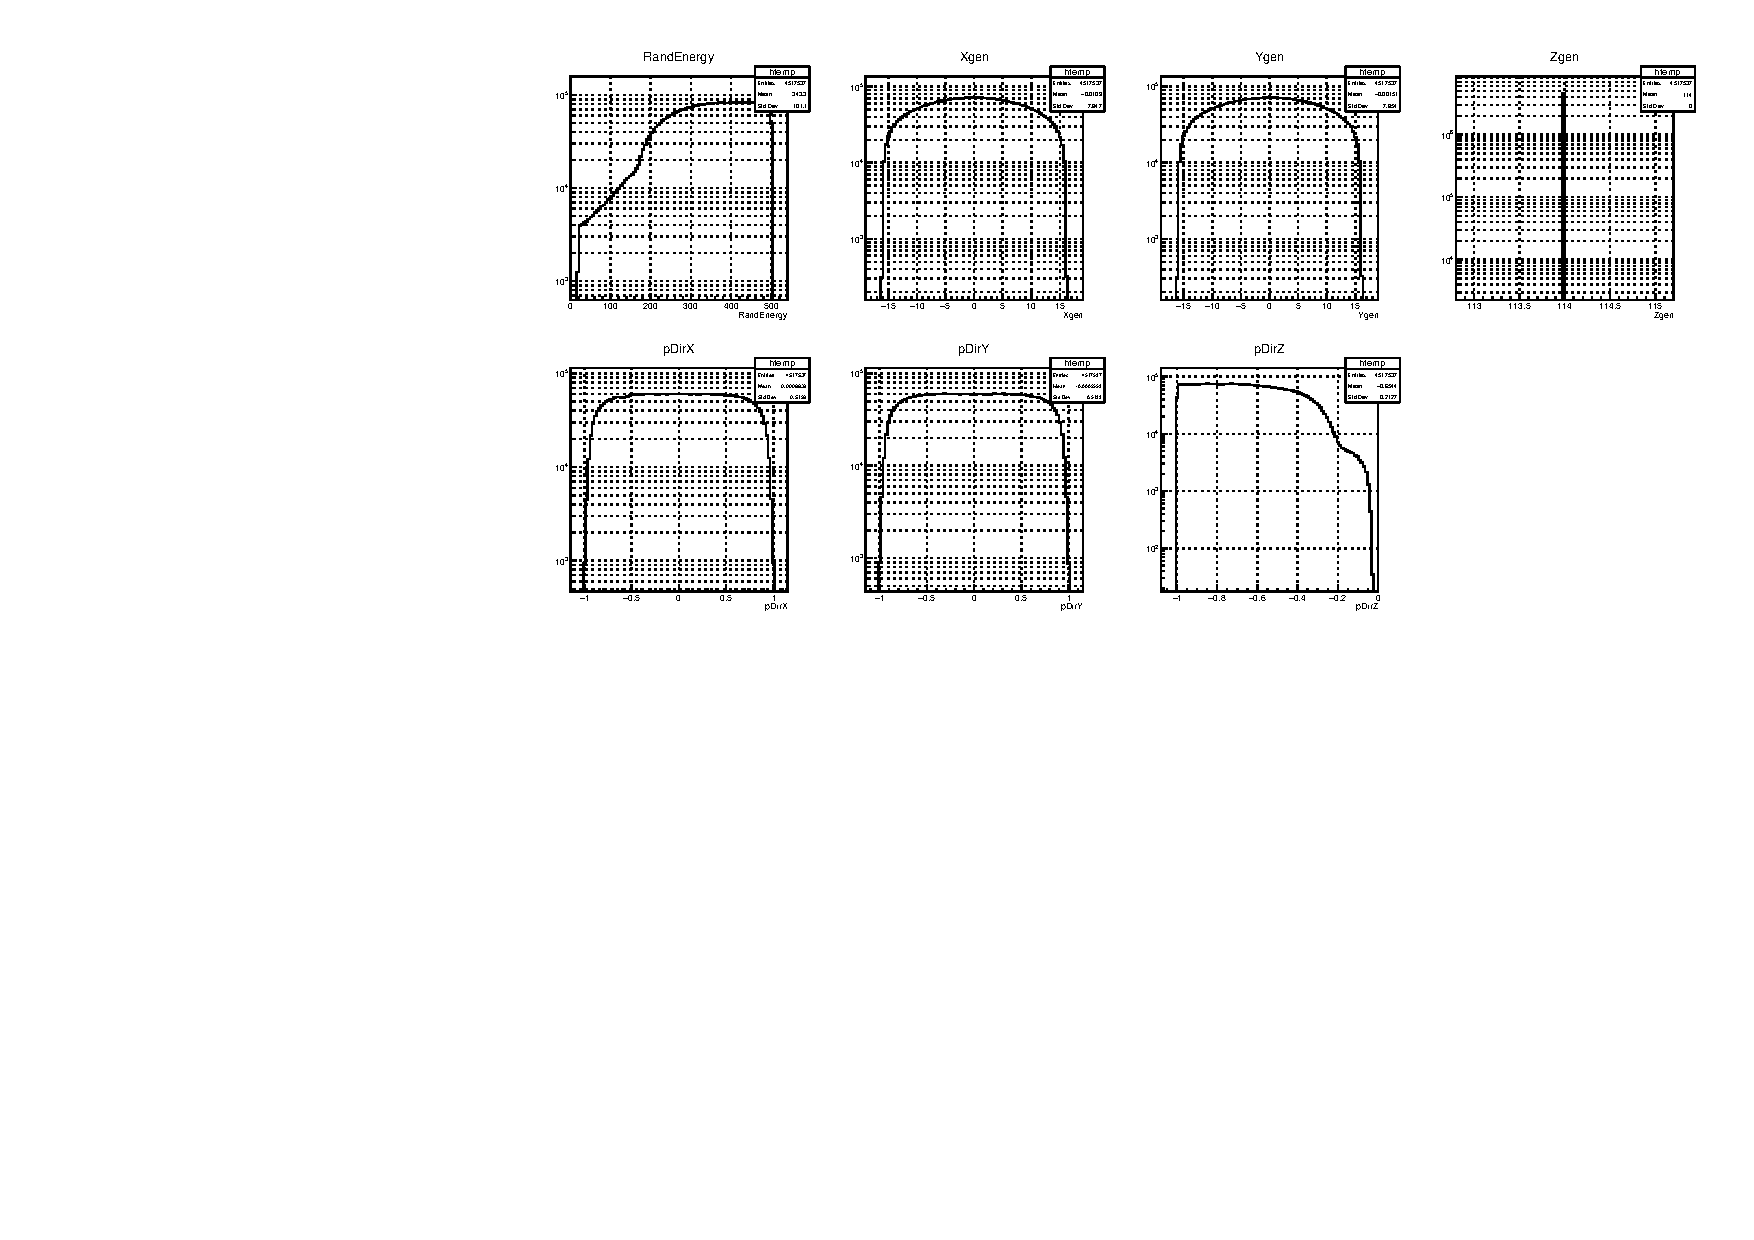
\includegraphics[width=0.8\textwidth]{/home/riccardo/Documenti/GeantProjects/LEM_GDML_upgrade/Output_Geant4Simulation_20230615_Old/Analysis_output/GDML_file_0/Montecarlo_alpha_t0.pdf}
            \caption{MC quantities}
        \end{figure}
        
        \end{frame}
        
        \begin{frame}
            \frametitle{Energies distribution for alphas}
        
        \begin{figure}[h]
            \centering
            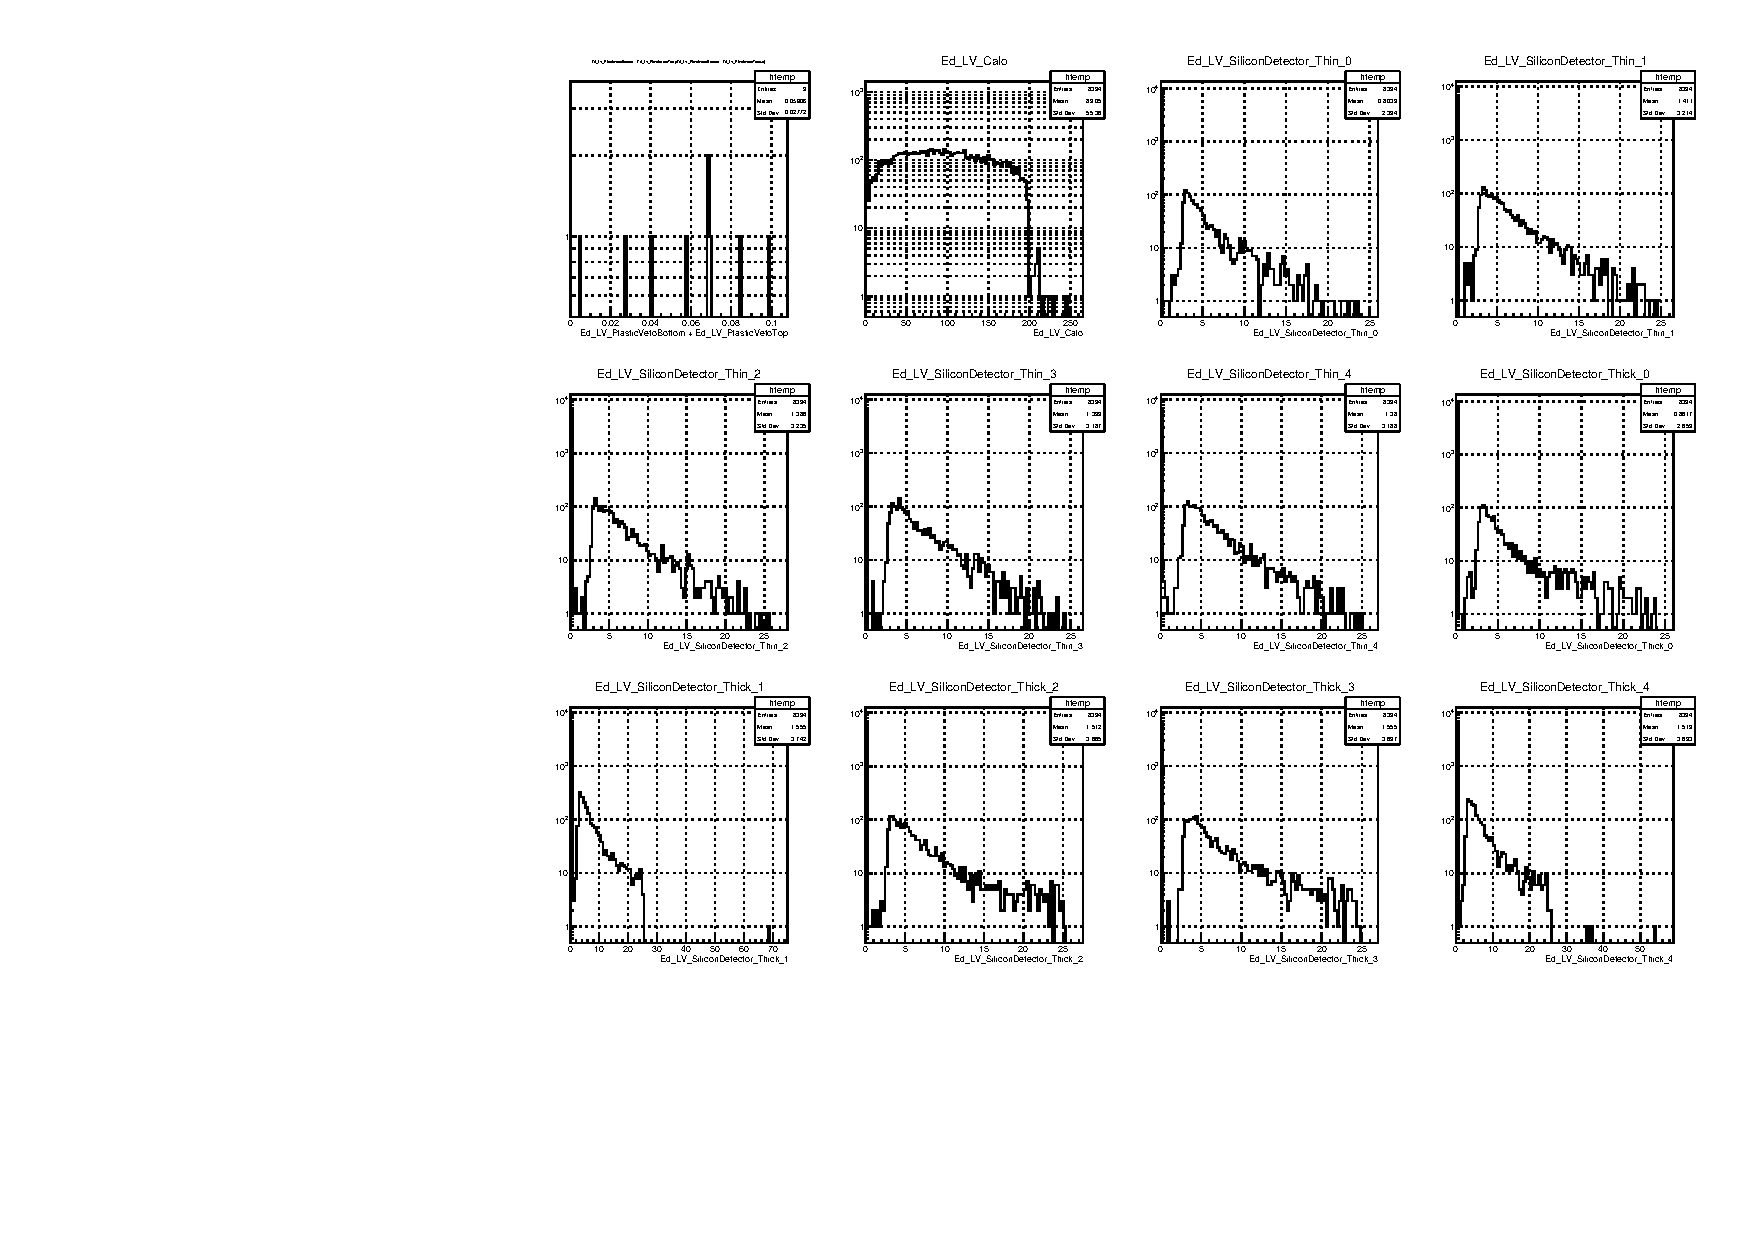
\includegraphics[width=0.8\textwidth]{/home/riccardo/Documenti/GeantProjects/LEM_GDML_upgrade/Output_Geant4Simulation_20230615_Old/Analysis_output/GDML_file_0/Energies_alpha_t0.pdf}
            \caption{Detected energies}
        \end{figure}
        
        \end{frame}
        
        \begin{frame}
            \frametitle{Angles distribution accepted for alphas}
        
        \begin{figure}[h]
            \centering
            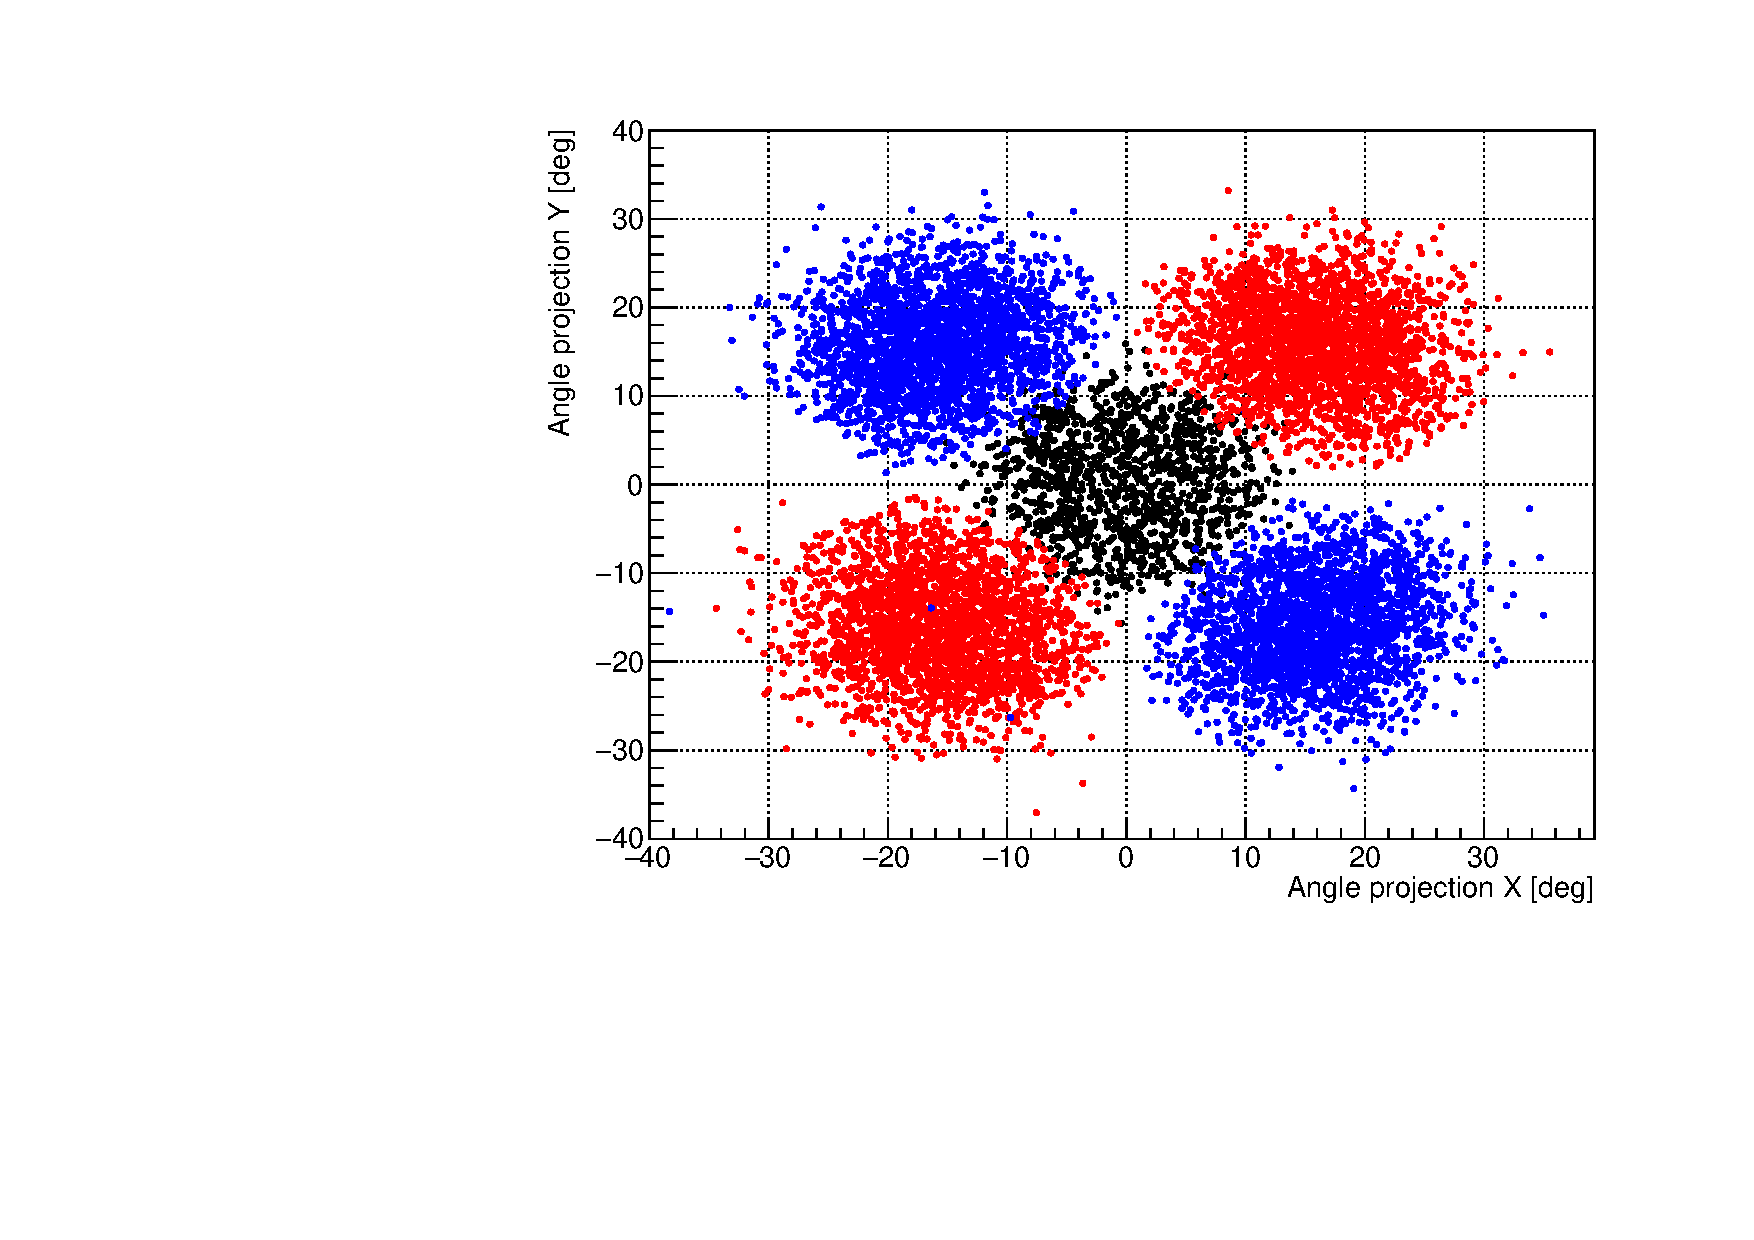
\includegraphics[width=0.8\textwidth]{/home/riccardo/Documenti/GeantProjects/LEM_GDML_upgrade/Output_Geant4Simulation_20230615_Old/Analysis_output/GDML_file_0/Angles_alpha_t0.pdf}
            \caption{Angles distribution}
        \end{figure}
        
        \end{frame}
        
        \begin{frame}
            \frametitle{Geometric factors for alphas}
        
        \begin{figure}[h]
            \centering
            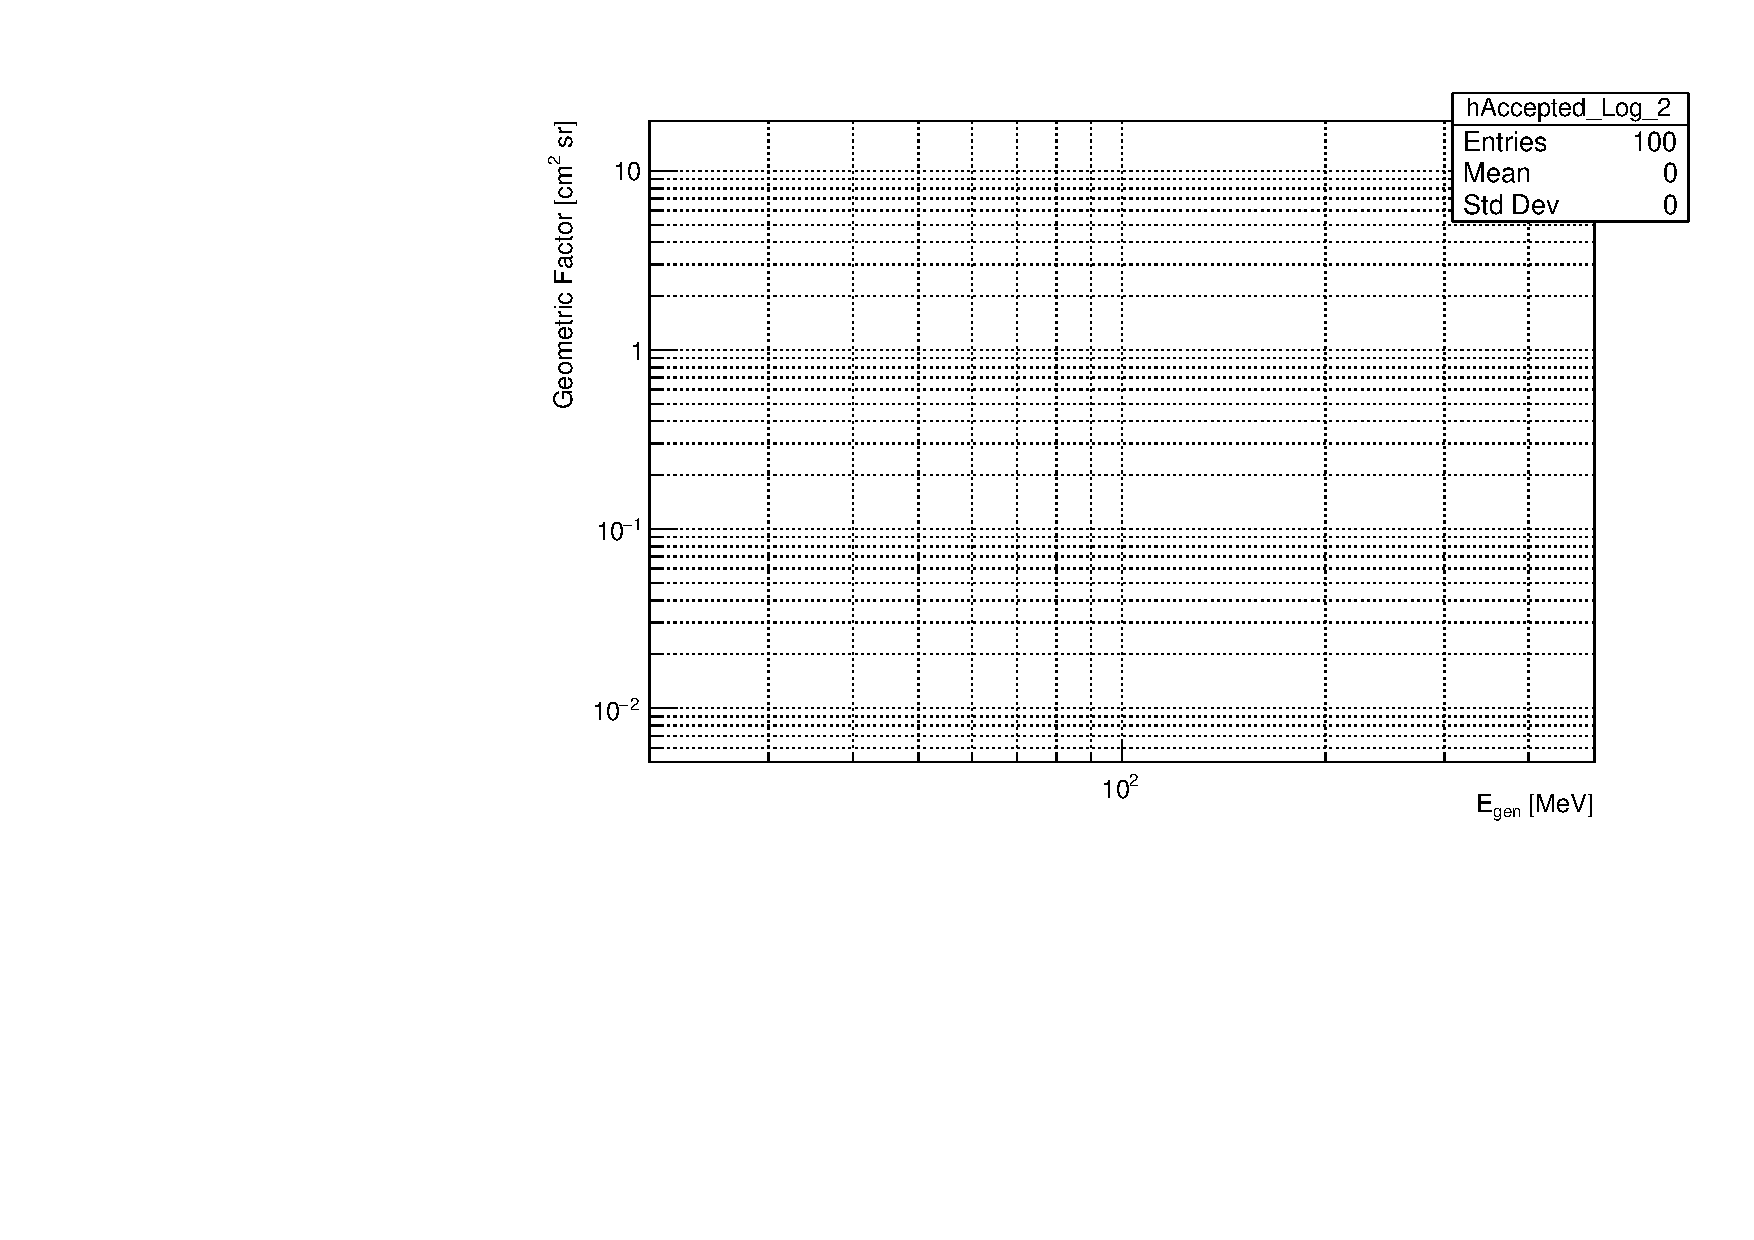
\includegraphics[width=0.8\textwidth]{/home/riccardo/Documenti/GeantProjects/LEM_GDML_upgrade/Output_Geant4Simulation_20230615_Old/Analysis_output/GDML_file_0/Acceptances_alpha_t0_alias.pdf}
            \caption{Geometric factors}
        \end{figure}
        
        \end{frame}
        
        \begin{frame}
            \frametitle{Geometric factors for alphas}
        
        \begin{figure}[h]
            \centering
            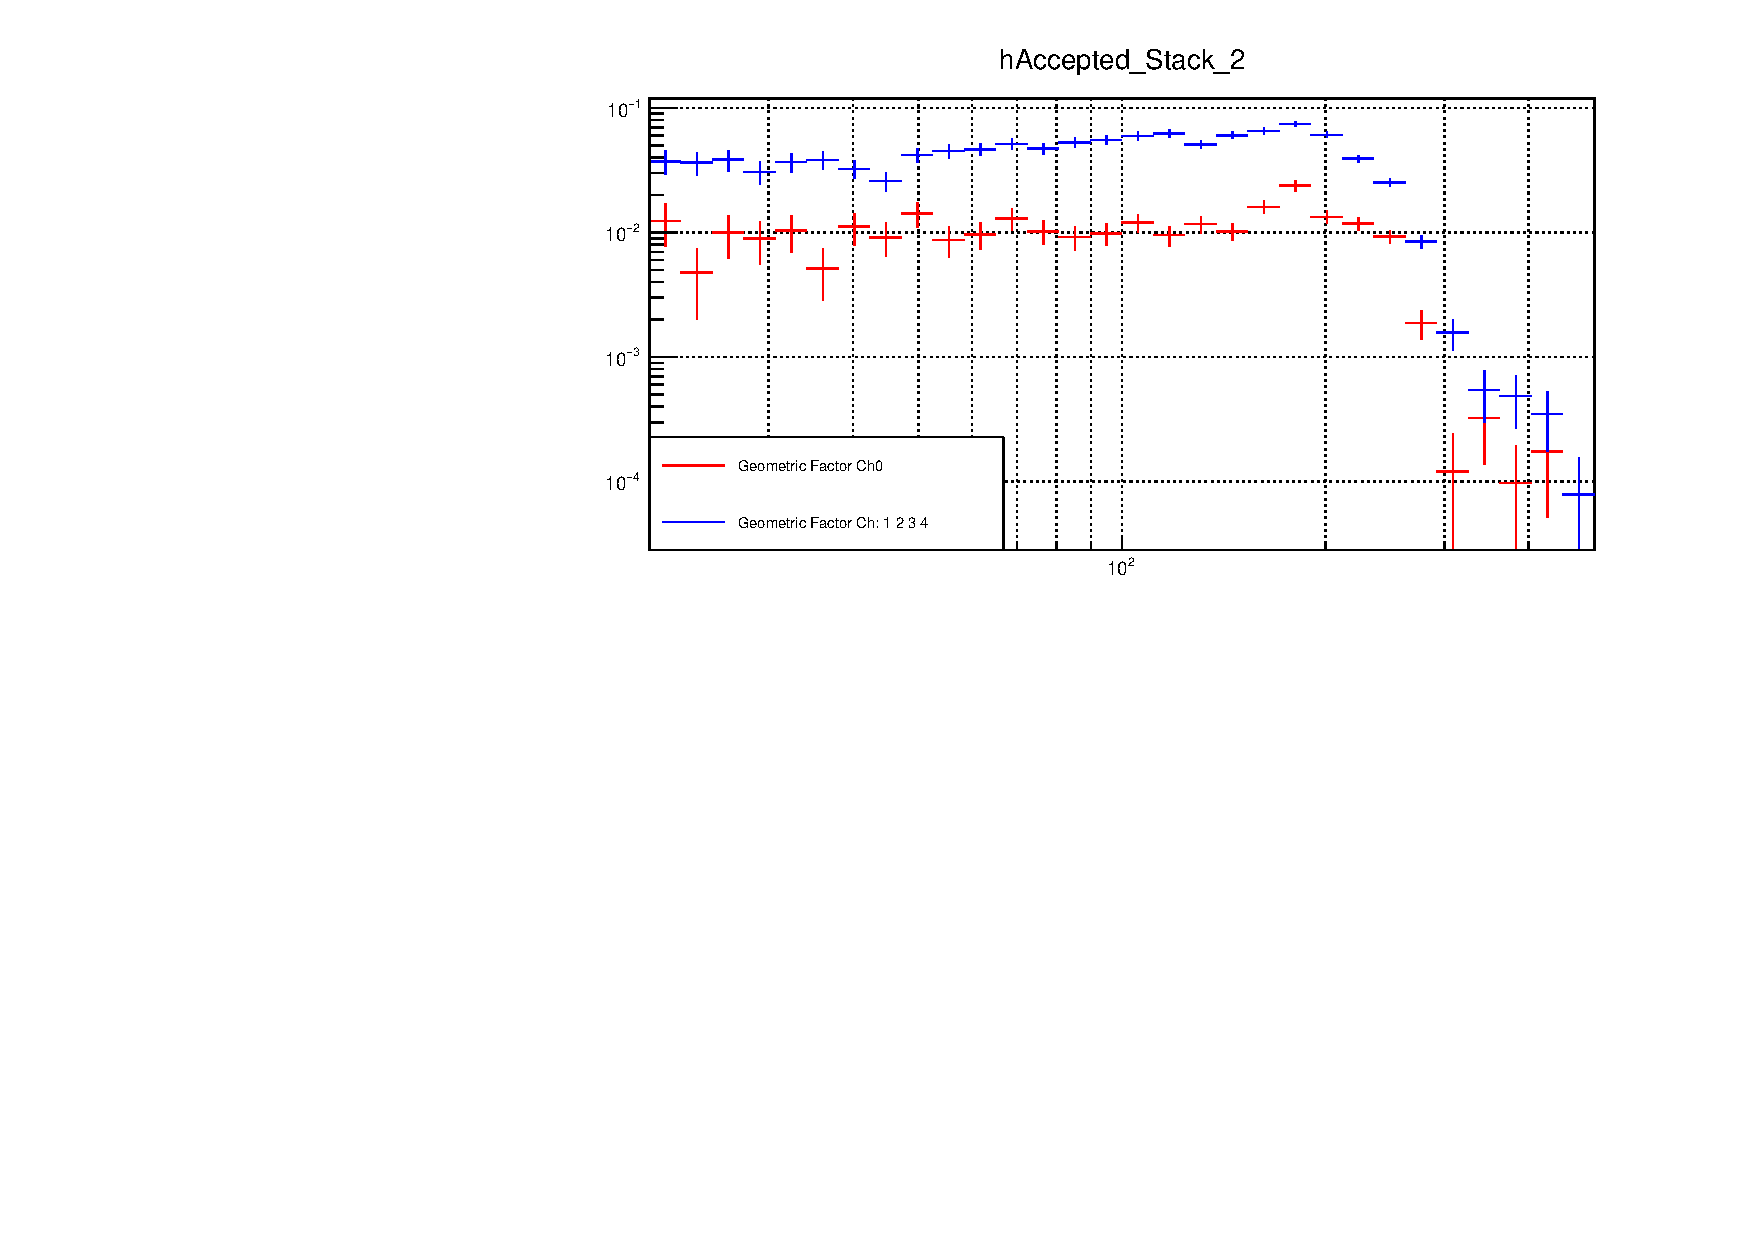
\includegraphics[width=0.8\textwidth]{/home/riccardo/Documenti/GeantProjects/LEM_GDML_upgrade/Output_Geant4Simulation_20230615_Old/Analysis_output/GDML_file_0/ChannelGeomFactor_alpha_t0_alias.pdf}
            \caption{Geometric factors}
        \end{figure}
        
        \end{frame}
        
        \begin{frame}
            \frametitle{Geometric factors for all particles}
        
        \end{frame}
        
        \end{document}
        